\chapter{Theoretical Background}
\section{Basics in Modeling Light in Computer Graphics}

\subsection{Radiometry}
One purpose of Computer Graphics is to simulate the interaction of light on a surface and how a real-world observer, such as a human eye, will perceive this. These visual sensations of an eye are modeled relying on a virtual camera which captures the emitted light from the surface. The physical basis to measure such reflected light depicts radiometry which is about measuring the electromagnetic radiation transfered from a soruce to a receiver. 

Fundamentally, light is a form of energy propagation, consisting of a large collection of photons, whereat each photon can be considered as a quantum of light that has a position, direction of propagation and a wavelength $\lambda$. A photon travels at a certain speed $v = \frac{c}{n}$, that depends only the speed of light $c$ and the refractive index $n$ through which it progrates. Its frequency is defined by $f = \frac{v}{\lambda}$ and its carried amount of energy $q$, mearsured in the SI unit Joule, is given by $q = hf= \frac{hv}{\lambda n}$ where $h$ is the Plank's constant. The total energy of a large collection of photons is hence $Q = \sum_i q_i$.

\subsection{Spectral Energy}

It is important to understand that the human eye is not equally sensitive to all wavelength of the spectrum of light and therefore responds differently to specific wavelengths. Remember that our goal is to model the human visual perception. This is why we consider the energy distribution of a light spectrum rather than considering the total energry of a photon collection since then we could weight the distribution according the human visual system. So the question we want to answer is: How is the energy distributed across wavelengths of light?

The idea is to make an energy histrogram from a given photon collection. For this we have to order all photons by their associated wavelength, discretize wavelength spectrum, count all photons which then will fall in same wavelength-interval, and then, finally, normalize each interval by the total energy $Q$. This will give us a histogram which tells us the spectral energy $Q_{\lambda}$ for a given discrete $\lambda$ interval and thus models the so called spectral energy distribution $\footnote{Intensive quantities can be thought of as density functions that tell the density of an extensive quantity at an infinitesimal point.}$.

\subsection{Spectral Power}
Rendering an image in Computer Graphics corresponds to capturing the color sensation of an illuminated, target scene at a certain point in time. As previousely seen, each color is associated by a wavelength and is directly related to a certain amount of enegry. In order to determine the color of a to-be-rendered pixel of an image, we have to get a sense of how much light (in terms of energy) passes through the area which the pixel corresponds to. One possibility is to consider the flow of energy $\Phi = \frac{\Delta Q}{\Delta t}$ transferred through this area over a small period of time. This allows us to measure the energy flow through a pixel during a certain amount of time. 

In general, power is the estimated rate of energy production for light sources and corresponds to the flux. It is measured in the unit Watts, denoted by Q. Since power is a rate over time, it is well defined even when energy production is varying over time. As with Spectral Energy for rendering, we are really interested in the spectral power $\Phi_\lambda = \frac{\Phi}{\lambda}$, measured in Watts per nanometer.

\subsection{Spectral Irradiance}
Before we can tell how much light is reflected from a given point on a surface towards the viewing direction of an observer, we first have to know how much light arrives at this point. Since in general a point has no length, area or even volume associated, let us instead consider an infinitimal area $\Delta A$ around a such a point. Then, we can ask ourself how much light falls in such a small area. When further observing this process over a short period in time, this quantity is the spectral irradiance $E$ as illustrated in figure $\ref{fig:irradiance}$. Summarized, this quantity tells us how much spectral power is incident on a surface per unit area and mathematically is equal:

\begin{equation}
 E = \frac{\Phi_{\lambda}}{\Delta A}
\end{equation} 

\begin{figure}[H]
  \centering
  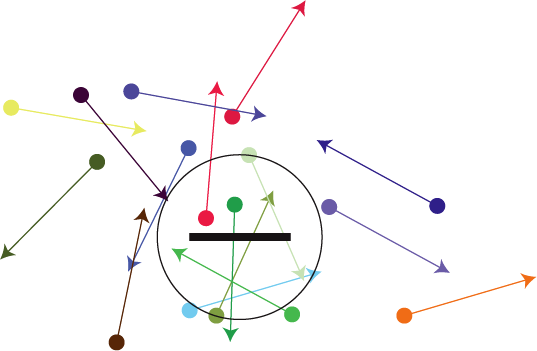
\includegraphics[scale=0.5]{background/irradiance.png}
  \caption{Irradiance is the summed up radiance over all directions}
  \label{fig:irradiance}
\end{figure}

\subsection{Spectral Radiance}
When rendering an image we have to determine the color of each pixel of the image. Although irradiance tells us how much light is arriving at a point as illustrated in figure $\ref{fig:irradiance}$, it tells us little about the direction that light comes from. This relates to how the human eye perceives the brightness of an illuminated objects when looking at it in a certain direction. 

\begin{figure}[H]
  \centering
  \subfigure[Radiances is the density of photons per area per solid angle]{
    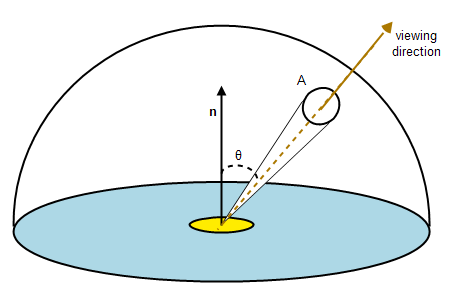
\includegraphics[scale=0.6]{background/radiancehemisphere.png}
    \label{fig:radiance}
  }
~
  \subfigure[Solid angle is the area of a surface patch on a sphere with radius R which is spanned by a set of directions]{  
    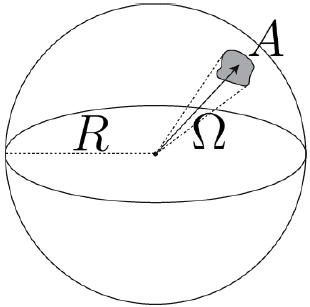
\includegraphics[scale=0.42]{background/solidangle.png}
    \label{fig:solidangle}
  }
  
\label{fig:radianceBasics}
\end{figure}s

This concepted is described by the radiometric quantity radiance. Basically, this is a measure of light energy passing through or is emitted off from a small area around a point on a surface towards a given direction during a short period in time. More formally this is the spectral power emerging from an arbitrary point (an infinitimal area around this point) and falls within a given solid angle (see figure$\footnote{Similar figute like used in computer graphics class 2012 in chapter colors}$ $\ref{fig:solidangle}$)in specific direction (usually towards the observer) as shown in figure $\ref{fig:radiance}$. Formally, this leads us to the following mathematical formalism: 

\begin{equation}
 L_{\lambda}(\omega) = \frac{d^2 \Phi_{\lambda}}{dA d\Omega} \approx \frac{\Phi_{\lambda}}{\Omega A}
\end{equation}

where $L$ is the observed spectral radiance in the unit energy per unit area per solid angle, which is $Wm^-2 sr^-1$ in direction $\omega$ which has an angle $\theta$ between the surface normal and $\omega$, $\Theta$ is the total flux or power emitted, $\theta$ is the angle between the surface normal and the specified direction, $A$ is the area of the surface and $\Omega$ is the solid angle in the unit steradian subtended by the observation or measurement.

It is useful to distinguish between radiance incident at a point on a surface and excitant from that point. Terms for these concepts sometimes used in the graphics literature are surface radiance $L_r$ for the radiance \textit{reflected} from a surface and field radiance $L_i$ for the radiance \textit{incident} at a surface.  

\subsection{BRDF}
In order to render the colorization of an observed object, a natural question in computer graphics is what portion of the reflected, incident light a viewer will receive, when he looks at an illuminated object. Therefore for any given surfaces which is illuminated from a certain direction $\omega_i$, we can ask ourself how much light is reflected off of any point on this surface towards a viewing direction $\omega_r$. This is where the Bidirectional Reflectance Distribution Function (short: BRDF) comes into play, which is a radiometric quantity telling us how much light is reflected at an opaque surface. Mathematically speaking, the BRDF is the ratio of the reflected radiance pointing to the direction $\omega_r$ to the incident irradiance comming from the inverse direction of $\omega_i$ as illustrated in figure $\ref{fig:brdfillustration}$. Hence the BRDF is a four dimensional function defined by four angles $\theta_i$, $\phi_i$, $\theta_r$ and $\phi_r$.

\begin{figure}[ht]
  \centering
  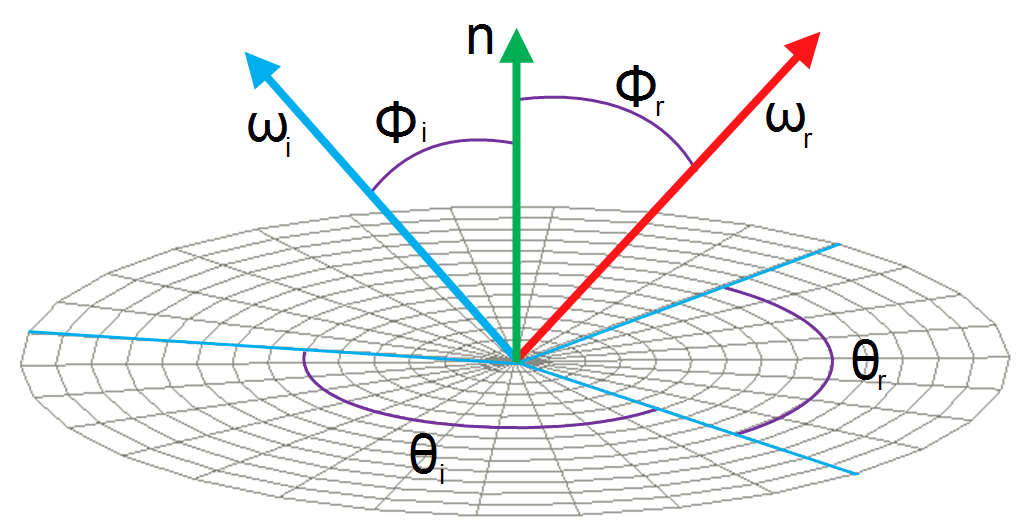
\includegraphics[scale=0.35]{background/mybrdfmodel.png}
  \caption[BRDF Model]{Illistration of the BRDF model, where $\omega_i$ is pointing to the light source and the existing direction is denoted by $\omega_r$. Both direction unit direction vectors defined w.r.t to a surface normal $\mathbf{n}$ for every point on the surface.}
  \label{fig:brdfillustration}  
\end{figure}

Which formally is for any given wavelength $\lambda$ equivalent to:

\begin{align}
  BRDF_{\lambda}(\omega_i, \omega_r)
  & = \frac{dL_r(\omega_r)}{dE_i(\omega_i)} \nonumber \\
  & = \frac{dL_r(\omega_r)}{L_i(\omega_i)cos(\theta_i)d\omega_i}
  \label{eq:defbrdf}
\end{align}

Where $L_{r}$ is the reflected spectral radiance, $E_i$ is the spectral irradiance and $\theta_{\text{i}}$ is the angle between $\omega_{\text{i}}$ and the surface normal $\mathbf n$. 

\subsection{Wavespectrum and Colors}
In order to see how crucial the role of human vision plays, let us consider the following definition of color by \textit{Wyszechkiu and Siles}$\footnote{mentioned in Computer Graphics Fundamentals Book from the year 2000}$ stating that \textit{Color is the aspect of visual perception by which an observer may distinguish differences between two structure-free fields of view of the same size and shape such as may be caused by differences in the spectral composition of the radiant energy concerned in the observation}. Therefore, similarly like the humans' perceived sensation of smell and taste, color vision is just another individual sense of perception giving us the ability to distinguish different frequency distribution of light experienced as color.

\begin{figure}[H]
  \centering
  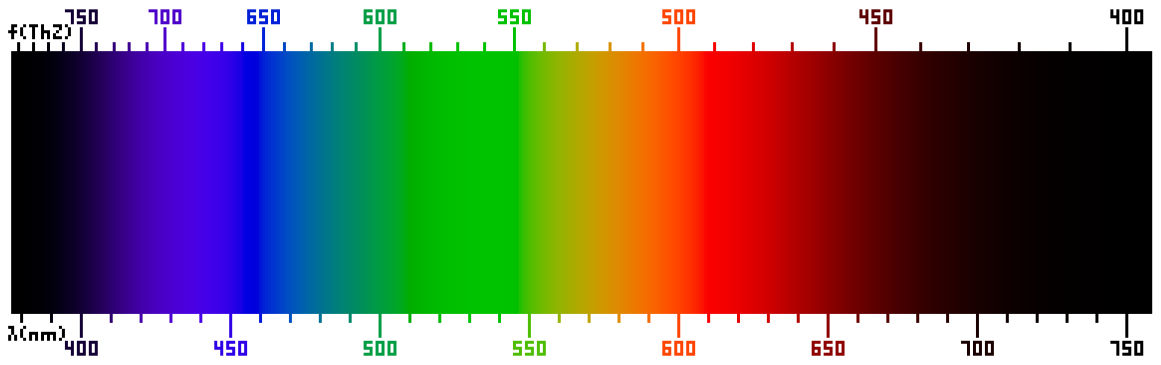
\includegraphics[scale=0.35]{background/lightspec.png}
  \caption[visiblelightspectrum]{Frequency (top) and wavelenght (bottom) of colors of the visible light spectrum$\footnotemark$.}
  \label{fig:colorspectrum}
\end{figure}
\footnotetext{Similar figute like used in computer graphics class 2012 in chapter colors}

In general an eye consists of photoreceptor cells which are responsible for providing ability of color-perception. A schematic of an eye is illustratied in figure $\ref{fig:humaneye}$. Basically, there are two specialized types of photoreceptor cells, cone cells which are responsible for color vision and rod cells, which allow an eye to perceive different brigthness levels.

\begin{figure}[H]
  \centering
  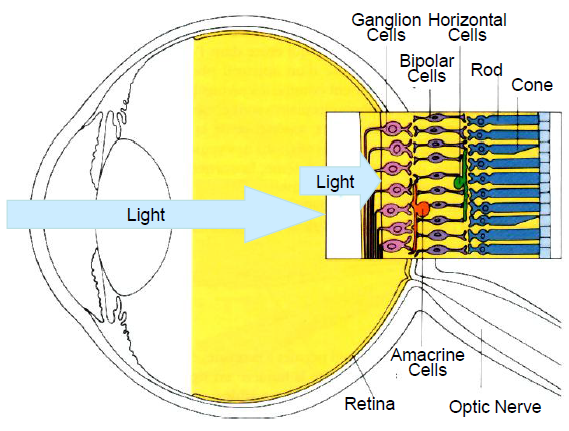
\includegraphics[scale=0.35]{background/humaneye.png}
  \caption[humanayeschematic]{Schematic$\footnotemark$ of photoreceptor cells, cones and rods, in human eye }
  \label{fig:humaneye}
\end{figure}
\footnotetext{image of illustration has been taken from \href{http://en.wikipedia.org/wiki/Bidirectional_reflectance_distribution_function}{wikipedia}}

A human eye is made of three different types of cone cells, having their peak sensivity in sensing color at different wavelength ranges. More precisely, there are cone cells most sensitive to short wavelengths which are between $420 nm$ and $440 nm$, those which are most sensitive in the middle range between $530 nm$ and $550 nm$ and those which have their peak in the long range, from $560 nm$ to $580 nm$. In principle, any color sensation in human color perception as shown in figure $\ref{fig:colorspectrum}$ can therefore be described by just three parameters, corresponding to levels of stimulus of the three types of cone cells.  

\subsection{Colorspace}
In order to render accurately images of how a human observer sees its world, a mathematical model of the human color perception is required. Remember that color sensation is due to a visual stimulus processed by cone cells in an eye. A human eye contains three different types of cone cells. Therefore, one possible approach is to describe each kind of these cone cells as a function of wavelength, returning a certain intensivity. In the early 1920, from a series of experiments the so called CIE XYZ color space was derived, describing response of cone cells of an average human individual, the so called standard observer. Basically, a statistically sufficiently large number of probands were exposed to different target light colors expressed by their wavelength. The task of each proband was to reproduce these target colors by mixing three given primary colors, red-, green- and blue-light. The strength  of each primary color could be manually adjusted by setting their relative intensivity. Those adjustment weights have been measured, aggregated and averaged among all probands for each primary color. This model describes each color as a triple of three real valued numbers$\footnote{note that there are  negative color weights possible in the CIE XYZ colors space. This is why some human perceived color sensations could not be reconstructed using just an additive color model (adding three positively weighted primary values). Therefore, a probabant was also allowed to move one of the primary colors to the target color and instead was supposed to reproduce this new color mix using the two remaining primaries (subtractive model). The value of the selected, moved primary was then interpreted as beeing negative weighted in an additive color model.}$, the so called tristimulus values.

Pragmatically speaking, color spaces describes the range of colors a camera can see, a printer can print or a monitor can display. Thus, formally we can define it as a mapping a range of physically produced colors from mixed light to an objective description of color
sensations registered in the eye of an observer in terms of tristimulus values. 

\begin{figure}[H]
  \centering
  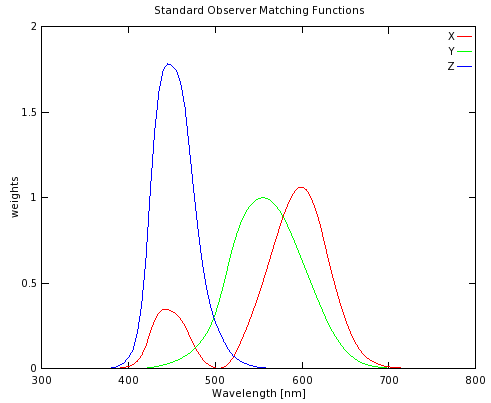
\includegraphics[scale=0.7]{background/somatchingfunctions.png}
  \caption{Plots of our color matching functions we used for rendering}
  \label{fig:matchingfunction}
\end{figure}

Interpolating all measured tristimuli values gives us three basis functions, the CIE color matching functions $\overline{x}(\lambda)$, $\overline{y}(\lambda)$, $\overline{z}(\lambda)$. In figure $\ref{fig:matchingfunction}$ are the numerical description of the chromatic response of the observer. They can be thought of as the spectral sensitivity curves of three linear light detectors yielding the CIE Tristimulus values X, Y and Z. 

The tristimulus values for a color with a spectral power distribution $I(\lambda)$, are given in terms of the standard observer by:

\begin{align}
    X= \int_{\Lambda} I(\lambda)\,\overline{x}(\lambda)\,d\lambda \nonumber \\
    Y= \int_{\Lambda} I(\lambda)\,\overline{y}(\lambda)\,d\lambda \nonumber \\
    Z= \int_{\Lambda} I(\lambda)\,\overline{z}(\lambda)\,d\lambda
\label{eq:tristimulusvalues}
\end{align}

Where $\lambda$, is the wavelength of the equivalent monochromatic light spectrum $\Lambda = [380nm, 780nm]$. Note taht it is not possible to build a display that corresponds to the CIE XYZ colorspace. For this reasons it is necessary to design other color spaces, which are physical realizable, offers efficient encoding, are perceptual uniform and have an intuitive color specification. There are simple conversions between XYZ color space, to other color space described as linear transformations.

\subsection{Spectral Rendering}
When rendering an image, most of the time we are using colors described in a certain RGB color space. However, a RGB colorspace results from a colorspace transformation of the tristimulus values, which themself are inherent to the human visual system. Therefore, many physically light phenomenon are poorly modeled when always relying on RGB colors for rendering. Using only RGB colors for rendering is alike we would assume that a given light source emits light of only one particular wavelength. But in reality this is barely the case. Spectral rendering is referring to use a certain wavelength spectrum, e.g. the human visible light spectrum, instead simply using the whole range of RGB values in order to render an illuminated scene. This captures the physical reality of specific light sources way more accurate. Keep in mind that, even when we make use of a spectral rendering approach, we have to convert the final spectra to RGB values, when we want to display an image on an actual display. 

\section{Wave Theory for Light and Diffraction}
\subsection{Basics in Wave Theory}
In order prepare the reader for physical relevant concepts used during later derivations and reasonings within this thesis, I am going to provide a quick introducation to the fundamental basics of wave theory and related concepts. In physics a wave describes a disturbance that travels from one location to another through a certain medium. The disturbance temporarly displaces the particles in the medium from their rest position which results in an energy transport along the medium during wave propagation. Usually, when talking about waves we are actually refering to a complex valued function which is a solution to the so called wave equation which is modeling how the wave disturbance proceeds in space during time. 

There are two types of waves, mechanical waves which deform their mediums during propagation like sound waves and electromagnetic waves consiting of periodic oscilations of an electromagnetic field such as light for example. Like simplified illustrated in figure $\ref{fig:wavebasics}$, there are several properties someone can use and apply in order to compare and distinguish different waves:

\begin{figure}[H]
  \centering
  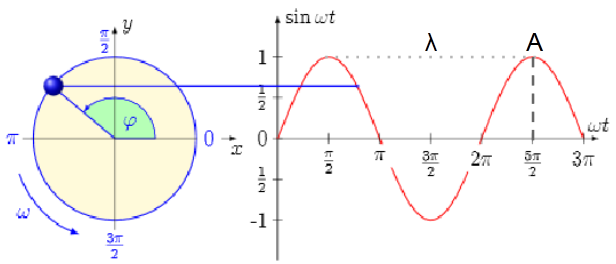
\includegraphics[scale=0.65]{background/waveschematicimpr.png}
  \caption[sinewave]{Simplified, one dimensionaly real valued wave function$\footnotemark$, giving an idea about some important wave properties. We denote the crest of a wave as the hightest point relative to the equilibrium line (zero height along time axis) and similarly the trough as the lowest point.}
  \label{fig:wavebasics}
\end{figure}
\footnotetext{Image source: http://neutrino.ethz.ch/Vorlesung/FS2013/index.php/vorlesungsskript}

\begin{description}
  \item[Wavelength:] Is usually denoted by $\lambda$ and is a measure for the spatial distance from one point to another until the shape of a wave repeats
  \item[Amplitude:] Is denoted by $A$ and there are two possible interprations: First, it is a measure of the height from the equilibrium point to the heighest point of a crest on the wave or the lowest point of a trough. This mean the amplitude can be positive or negative. However, usually, someone is  just interested the absolute value of an amplitude, the magnitude of a wave. For light waves it is a relative measure of intensity or brightnes to other lught waves of the same wavelength. And secondly, it can be interpreted as a measure how much energy a wave carries wherate the greater the absoulte aplitute value, the bigger the amount of energy being carried.
  \item[Frequency:] Is a measure of the number of waves which are passing through a particular point in the propagation medium during a certain time and is denoted by $f$.
  \item[Phase:] Is denoted by $\phi$. Describes either the offset of initial position of a wave or the relative displacement between or among waves having the same frequency. Two waves two waves with same frequency are denoted by being in phase if they have the same phase. This means they line up everywhere. As a remark, we denote by $\omega$ the angular frequency which is equal $2\pi f$. 
\end{description}

A geometrical property of waves is their wavefront. This is either a surface or line along the path of wave propagation on which the disturbance at every point has the same phase. Three are basically three types of wavefronts: spherical-, cylindrical- and plane wavefront. If point in a isotropic medium is sending out waves in three dimensions, then the coresponding wavefronts are spheres, centered on the source point. Hence spherical wavefront is the result of a spherical wave, also denoted as a wavelet. Note that for electromagnetic waves, the phase is a poisition of a point in time on a wavefront cycle (motion of wave over a whole wavelength) whereat a complete cycle is defined as being equal 360 degrees.



\subsection{Wave Interference}
Next, after having seen that a wave is simply a traveling disturbance along a medium, having some special properties, someone could ask what happens when there are several waves travaling on the same medium. Especially, we are interested how these waves will interac with each other. In physics we use the term interference for the resulting phenomenon when two or more waves meet. Hence interference is the interaction of waves when they encounter each other at a point along their medium of propagation. At each point where two waves superpose, their total displacement at these points is the sum of the displacements of each indiviudal wave at those points. Then, the resulting wave is having a greater or lower amplitude than each seperate wave and this we can interprete the interference as the addition operator for waves. Two extreme scenarios are illustrated in figure $\ref{fig:interferenceconcept}$. There are basically three variants of interferences which can occur, depending on how crest and troughs of the waves are matched up:

\begin{figure}[H]
  \centering
  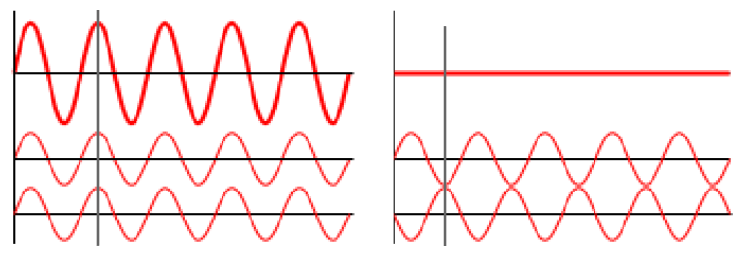
\includegraphics[scale=0.65]{background/interferenceconcept.png}
  \caption[interference]{Interference scenarios$\footnotemark$ when two waves waves meet: On the left handside, there is constructive interference and on the right handside there is destructive interference illustrated.}
  \label{fig:interferenceconcept}
\end{figure}
\footnotetext{Image source: \texttt{http://en.wikipedia.org/wiki/Interference\textunderscore(wave\textunderscore propagation)} } 

\begin{itemize}
  \item Either a crest of a wave meets a crest of another wave or similarly a trough meets a trough of another wave. This scenario is denoted as constructive interference and occurs at any location along the medium where the two interfering waves have a displacement in the same direction. This is equivalent like saying that the phase difference between the waves is a multiple of $2\pi$. Then the resulting amplitude at that point is being much larger than the amplitude of an individual wave. For two waves with an equal amplitude interfering constructively, the resulting amplitude is twice as large as the amplitude of an individual wave.
  \item Either a crest of a wave meets a trough of another wave or vice versa. This scenario is denoted as destructive interference and occurs at any location along the medium where the two interfering waves have a displacement in the opposite direction. This is like saying that the phase difference between the waves is an odd multiple of $\pi$. Then the waves completely cancel each other out at any point they superimpose.
  \item If the phase difference between two waves is intermediate between the first two scenarios, then the magnitude of the displacement lies between the minimal and maximal values which we could get from constructive interference.
\end{itemize}

\subsection{Wave Coherence}
\subsubsection{Concept of Coherence}
When considering waves which are traveling on a shared medium along the same direction, we could examine how their phase difference is changing over time. Formulating the changement of their relative phase as a function of time will provides us a quantitative measure of the synchronism of two waves, the so called wave coherence. In order to better understand this concept, let us consider a perfectly mathematical sine wave and second wave which is a phase-shifted replica of the first one. A property of mathematical waves is that they keep their shape over an infinity amount of moved wavelengths. In our scenario, both waves are traveling along the same direction on the same medium, like exemplarily illustrated in figure $\ref{fig:coherencesinsignal}$.
\begin{figure}[H]
  \centering
  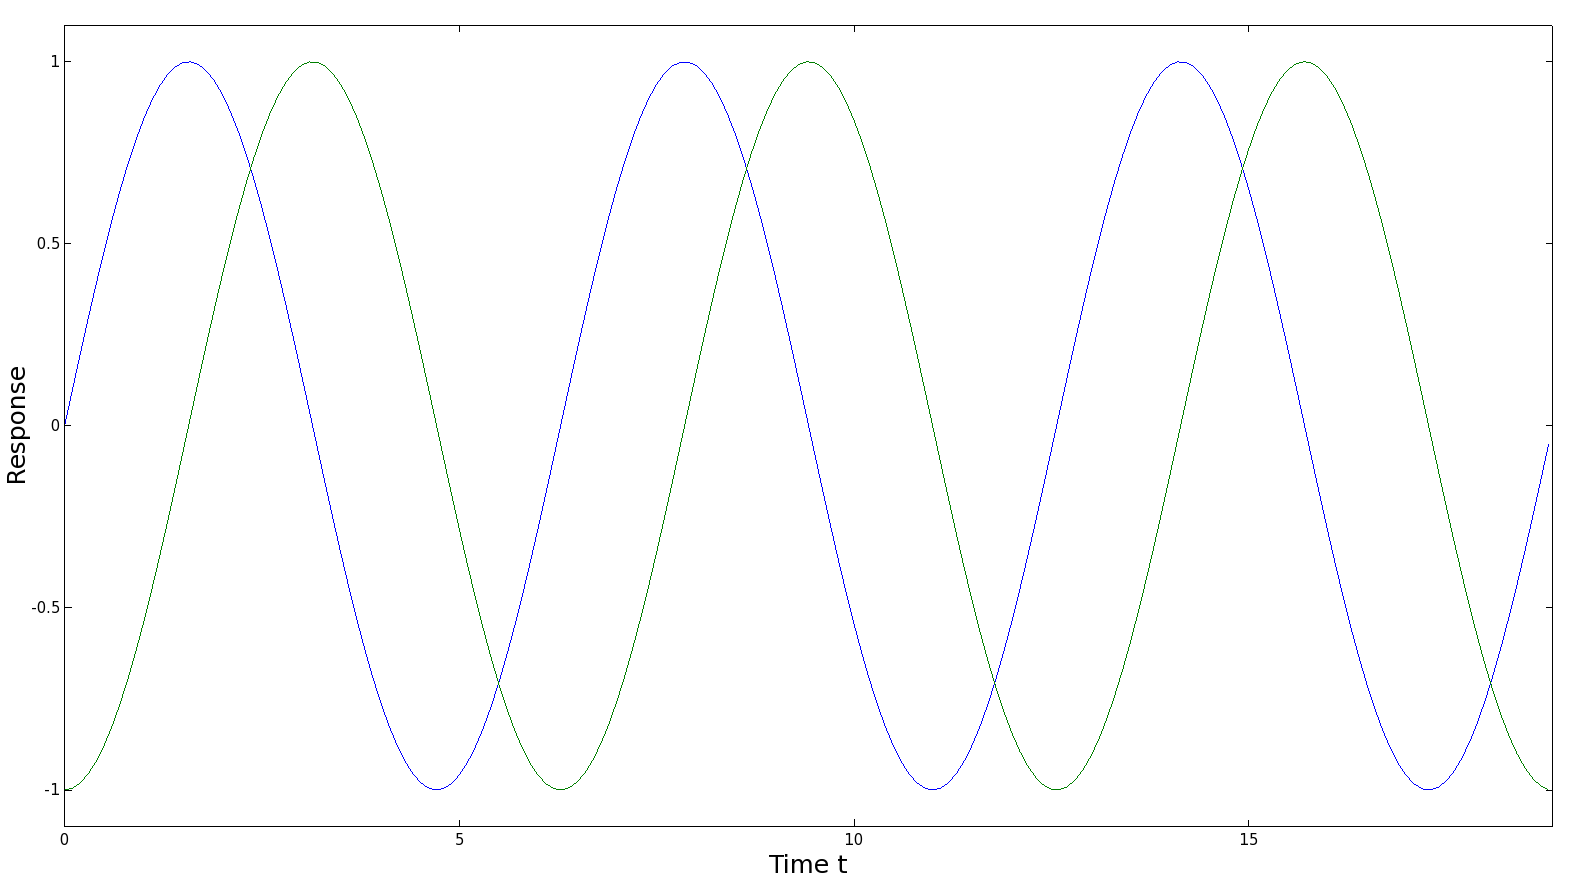
\includegraphics[scale=0.3]{background/coherencesinsignal.png}
  \caption{Two mathematical sine waves which are perfectly coherent which means that their phase difference is constant for every point in time.}
  \label{fig:coherencesinsignal}
\end{figure}

Taking the difference between the two sine waves from the previous figure yields always a constant number. Therefore, those two waves are said to be coherent and hence perfectly synchronous over time. Notice that this scenario is completly artificial since in nature there are no mathematical sine waves. Rather, the phase difference is then a fuction of time $p(t)$. The more coherent two waves are, the slower this function will change over time. 
In fact, two waves are said to be coherent if they are either of the same frequency, temporally in phase or have the same amplitude at every point in time.
Thus two waves are coherent if they are generated at the same time, having the same frequency, amplitude, and phase. Reversely, Waves are considered incoherent or also asynchronous if they have no stable phase difference. This means $p(t)$ is heavly varying over time. Coherence describes the effect of whether waves will tend to interfere with each other constructively or destructively at a certain point in time and space. Thus this is a property of waves that enables stationary interference. The more correlated two waves are, the higher their degree of coherence is. In physics coherence between waves is quantified by the corss-correlation function, which basically predicts the value of a second wave using the value of the first one. There are two basic coherence classifications:

\begin{itemize}
  \item Spatial coherence is dealing with the question of what is the range of distance between two points in space in the extend of a wave for which there is occuring a significant effect of interference when averaged over time. This is formally answered by considering the correlation between waves at different point in space. The range of distance is also denoted as the coherence area.
  \item Temporal coherence examines the ability of how well a wave will interfer with itself at different moments in time. Mathematically, this kind of coherence is computed by averaging the measured correlation between the value of the wave and the delayed version of itself at different pairs of time. The Coherence time denotes the time for which the propagating wave is coherent and we therefore can predict its phase using the correlation function. The distance a wave has traveled during the coherence time is denoted as the coherence length.
\end{itemize}

\subsubsection{Derivation}
inject contribution here

\subsection{Huygen's Principle}
\begin{figure}[H]
  \centering
  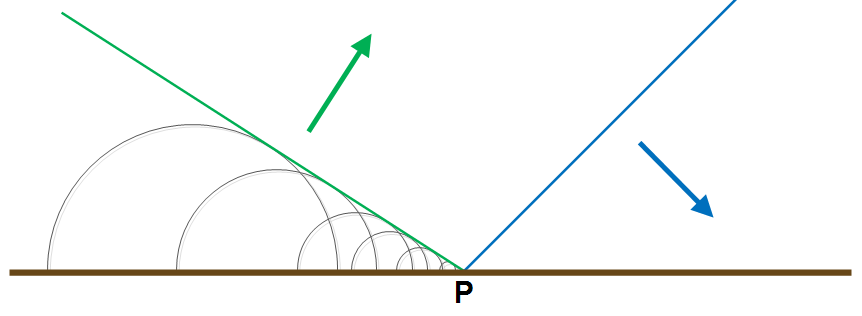
\includegraphics[scale=0.6]{background/huygensprinciple.png}
  \caption[Huygen's Principle]{A moving wavefront (blue) encounters an obstacle (a surface in brown colors) and produces a new wavefront (green) as a result of superposition among all secondary wavelets.}
  \label{fig:huygensprinciple}
\end{figure}


\subsection{Diffraction Gratings}
\subsection{Waves Diffraction}

\section{Stam's BRDF formulation}
\label{sec:sumstam}
In his paper about Diffraction Shader, J. Stam derives a BRDF which is modeling the effect of diffraction for various analytical anisotropic reflexion models relying on the so called scalar wave theory of diffraction for which a wave is assumed to be a complex valued scalar. 
It's noteworthy, that Stam's BRDF formulation does not take into account the polarization of the light. Fortunately, light sources like sunlight and light bulbs are unpolarized. 

A further assumption in Stam's Paper is, the emanated waves from the source are stationary, which implies the wave is a superposition of independent monochromatic waves. This implies that each wave is associated to a definite wavelength lambda. However, sunlight once again fulfills this fact.

In our simulations we will always assume we have given a directional light source, i.e. sunlight. Hence, Stam's model can be used for our derivations.

For his derivations Stam uses the Kirchhoff integral (ADD REF TO WIKI), which is relating the reflected field to the incoming field. This equation is a formalization of Huygen’s well-known principle that states that if one knows the wavefront at a given moment, the wave at a later time can be deduced by considering each point on the first wave as the source of a new disturbance. Mathematically speaking, once the field  $\psi_1 =  e^{ik\mathbf{x} \cdot \mathbf{s}\mathbf{s}}$ on the surface is known, the field $\psi_2$ everywhere else away from the surface can be computed.
More precisely, we want to compute the wave $\psi_2$ equal to the reflection of an incoming planar monochromatic wave $\psi_1 = e^{ik \omega_i * x}$  traveling in the direction $\omega_i$ from a surface $S$ to the light source. Formally, this can be written as:

\begin{equation}
\psi_{2}(\omega_i, \omega_r) = \frac{i k e^{i K R}}{4 \pi R} (F(-\omega_i-\omega_r)-(-\omega_i+\omega_r)) \cdot I_{1}(\omega_i, \omega_r) 
\label{eq:kirchhoff}
\end{equation}

with

\begin{equation}
I_{1}(\omega_i, \omega_r) = \int_{S} \hat{\mathbf{n}} e^{ik(-\omega_i-\omega_{r}) \cdot \mathbf{s} d\mathbf{s}}
\label{eq:IBase}
\end{equation}

In applied optics, when dealing with scattered waves, one does use differential scattering cross-section rather than defining a BRDF which has the following identity: 

\begin{equation}
    \sigma^0 = 4 \pi \lim_{R \to \infty} R^2 \frac{\langle \left|\psi_2\right|^2\rangle}{\langle \left|\psi_1\right|^2\rangle}
\end{equation}

where R is the distance from the center of the patch to the receiving point $x_p$, $\hat{\mathbf{n}}$ is the normal of the surface at s and the vectors:

The relationship between the BRDF and the scattering cross section can be shown to be equal to 

\begin{equation}
 BRDF = \frac{1}{4\pi}\frac{1}{A}\frac{\sigma^0}{cos(\theta_i)cos(\theta_r)}
 \label{fig:crossscateringbrdfrelationship} 
\end{equation}

where $\theta_i$ and $\theta_r$ are the angles of incident and reflected directions on the surface with the surface normal $n$. See ~\ref{fig:geometricsetup}.

\begin{figure}[ht]
  \centering
  
\includegraphics[scale=0.25]{brdfdiagram.png}
  \caption{$\omega_i$ points toward the light source, $\omega_r$ points toward the camera, $n$ is the surface normal}
  \label{fig:geometricsetup}  
\end{figure}

The components of vector resulting by the difference between these direction vectors:
In order to simplify the calculations involved in his vectorized integral equations, Stam considers the components of vector 
\begin{equation}
  (u,v,w) = -\omega_i - \omega_r 
\label{eq:uvw}
\end{equation}

explicitly and introduces the equation: 
\begin{equation}
  I(ku,kv) = \int_{S} \hat{\mathbf{n}} e^{ik(u,v,w) \cdot \mathbf{s} d\mathbf{s}} 
\label{eq:Istart}
\end{equation}

which is a first simplification of $\ref{eq:IBase}$. Note that the scalar $w$ is the third component of ~\ref{eq:uvw} and can be written as $w = -(cos(\theta_i)+cos(\theta_r))$ using spherical coordinates. The scalar $k=\frac{2\pi}{\lambda}$ represent the wavenumber.


During his derivations, Stam provides a analytical representation for the Kirchhoff integral assuming that each surface point $s(x,y)$ can be parameterized by $(x,y,h(x,y))$ where $h$ is the height at the position $(x,y)$ on the given $(x,y)$ surface plane. Using the tangent plane approximation for the parameterized surface and plugging it into $\ref{eq:Istart}$ he will end up with: 

\begin{equation}
    \mathbf{I}(ku, kv) = \int \int (-h_{x}(x,y), -h_{y}(x,y), 1) e^{ikwh(x,y)} e^{ik(ux + vy)} dx dy
\label{eq:I1}
\end{equation}

For further simplification Stam formulates auxillary function which depends on the provided height field: 
\begin{equation}
  p(x,y) = e^{iwkh(x,y)} 
\label{eq:px}
\end{equation}

which will allow him to further simplify his equation $\ref{eq:I1}$ to:

\begin{equation}
    \mathbf{I}(ku, kv) = \int \int \frac{1}{ikw}(-p_x, -p_y, ikwp) dx dy
\label{eq:I2}
\end{equation}

where he used that $(-h_{x}(x,y), -h_{y}(x,y), 1)e^{kwh(x,y)}$ is equal to $\frac{(-p_x, -p_y, ikwp)}{ikw}$ using the definition of the partial derivatives applied to the function $\ref{eq:px}$.

Let $P(x,y)$ denote the Fourier Transform (FT) of $p(x,y)$. Then, the differentiation with respect to x respectively to y in the Fourier domain is equivalent to a multiplication of the Fourier transform by $-iku$ or $-ikv$ respectively. This leads him to the following simplification for $\ref{eq:I1}$:

\begin{equation}
    \mathbf{I}(ku, kv) = \frac{1}{w}P(ku, kv) \cdot (u,v,w)
\label{eq:I3}
\end{equation}

Let us consider the term $g = (F(-\omega_i - \omega_r)-(-\omega_i + \omega_r))$, which is a scalar factor of $\ref{eq:kirchhoff}$. The dot product with $g$ and $(-\omega_i - \omega_r)$ is equal $2F(1 + \omega_i \cdot \omega_r)$. Putting this finding and the identity $\ref{eq:I3}$ into $\ref{eq:kirchhoff}$ he will end up with:

\begin{equation}
\psi_{2}(\omega_i, \omega_r) = \frac{i k e^{i K R}}{4 \pi R} \frac{2F(1 + \omega_i \cdot \omega_r)}{w} P(ku, kv)
\label{eq:kirchhoffFinding}
\end{equation}

By using the identity $\ref{fig:crossscateringbrdfrelationship}$, this will lead us to his main finding:
\begin{equation} 
  BRDF_{\lambda}(\omega_i, \omega_r) = \frac{k^2 F^2 G}{4\pi^2 A w^2} \langle \left|P(ku, kv)\right|^2\rangle
\label{eq:mainstam}
\end{equation}

where $G$ is the so called geometry term which is equal: 

\begin{equation}
  G =\frac{(1 + \omega_i \cdot \omega_r)^2}{cos(\theta_i)cos(\theta_r)}
\label{eq:geometricterm}
\end{equation}

